\subsection{Zernike Polynomials}

The Fourier series is very convenient to define periodic functions. But for functions that are defined on a disc, we will need a different way. The Zernike polynomials are a sequence of polynomials that are orthogonal on the unit disc. They play important roles in various optics branches such as beam optics and imaging. We will make use of the properties of Zernike polynomials to define toroidal cross-section. For the Fourier series, we used a single parameter $n$, for the Zernike Polynomials, we will use 2 parameters $l$ and $m$. Again, by dividing sine and cosine terms, we can show odd and even Zernike Polynomials as,
\begin{equation}
    \mathcal{Z}_l^m(\rho,\theta) = \begin{cases}\begin{aligned}
            &\mathcal{R}_l^{m}(\rho) cos(m\theta) & \text{for } m\geq 0 \text{ and } 0\leq\rho\leq 1 \\[.3cm]
            &\mathcal{R}_l^{|m|}(\rho) sin(|m|\theta) & \text{for } m < 0  \text{ and } 0\leq\rho\leq 1
        \end{aligned}
    \end{cases}
    \label{zernike-poly}
\end{equation}
where $\mathcal{R}_l^m$ is the radial part of the Zernike Polynomials and it is defined as,
\begin{equation}
    \mathcal{R}_l^{m} (\rho) = \mathlarger{\mathlarger{\sum}}_{s=0}^{(l-m)/2} \frac{(-1)^s(l-s)!}{ s!\left( \cfrac{l+m}{2} - s\right)! \left( \cfrac{l-m}{2} + s\right)!  }\hspace{0.1cm} \rho^{l-2s} \hspace{1cm}\text{for } m\geq0  \text{ and } 0\leq\rho\leq 1
\end{equation}
First few of the radial part Zernike Polynomials are,
\begin{figure}[H]
    \centering
    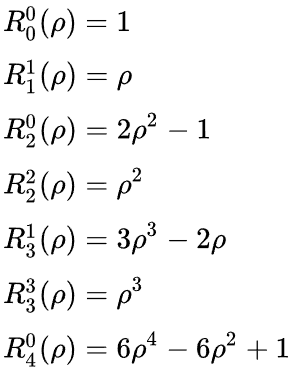
\includegraphics[height=4cm]{figures/zernike-poly.png}
\end{figure}
So, we can write, for example, even Zernike Polynomials in full form as,

\begin{equation}
    \mathcal{Z}_l^m(\rho,\theta) = cos(m\theta) \mathlarger{\mathlarger{\sum}}_{s=0}^{(l-m)/2} \frac{(-1)^s(l-s)!}{ s!\left( \cfrac{l+m}{2} - s\right)! \left( \cfrac{l-m}{2} - s\right)!  }\hspace{0.1cm} \rho^{l-2s} \hspace{1cm}\text{for } m\geq0  \text{ and } 0\leq\rho\leq 1
\end{equation}

Notice that $(l-m)/2$ must be a positive integer. Therefore, possible values for m are $m= \{-l, -l+2, ..... , l-2, l\}$. For odd $l$ values, for example $l=3$, $m=\{-3, -1, 1, 3\}$, and for even $l$ values, for example $l=4$, $m = \{-4, -2, 0, 2, 4\}$. Moreover, for $\rho$ = 0, these polynomials don't depend on $\theta$ (as it should be). For $m$=0, this is trivial [cos($0.\theta$)=1]. If $|m|>0$, $l-2s = l-2\frac{l-|m|}{2} = |m| > 0$, will always satisfy that there is $\rho$ to some positive power, which in turn when evaluated at $\rho = 0$, gives 0. Therefore, we can say that,
\begin{equation}
    \mathcal{Z}_l^m(\rho=0,\theta) = \mathcal{R}_l^0(0) = \begin{cases}
        0 & \text{if m is 0, $l$ must be even number, so odd $l$ values are 0}\\
        (-1)^{l/2}  & \text{products of 4 are 1, others -1}
    \end{cases} \label{zernike-at0}
\end{equation}
The radial part Zernike Polynomials can also be calculated as,
\begin{equation}
    \mathcal{R}_l^m(\rho) = (-1)^{(l-m)/2} \rho^m  P_{(l-m)/2}^{m, 0} (1 - 2 \rho^2)
\end{equation}
where $P_{n}^{\alpha, \beta}(\rho)$ is a Jacobi polynomial. This allows numerical simulations to use stable recurrence relations for the Jacobi polynomials. Since Jacobi polynomials have their recursion relation, we can avoid many calculations. Here is the recursion relations for Jacobi polynomials,
\begin{equation}
    2n(c-n)(c-2)P_{n}^{\alpha,\beta}(\rho) = (c-1)[c(c-2)\rho + (a-b)(c-2n)]P_{n-1}^{\alpha,\beta}(\rho) - 2(a-1)(b-1)cP_{n-2}^{\alpha,\beta}(\rho)
\end{equation}
where,
\begin{equation}
    c = 2n + \alpha + \beta, \hspace{1cm} a = n +\alpha, \hspace{1cm} b = n + \beta
\end{equation}
For the calculation of derivatives, we will be using the following relation,
\begin{equation}
    \frac{d^k}{dx^k} P_n^{(\alpha, \beta)}(x) = \frac{\Gamma(\alpha + \beta + n + 1 + k)}{2^k\Gamma(\alpha + \beta + n + 1)} P_{n-k}^{(\alpha + k, \beta + k)}(x)
\end{equation}

Just as in the Fourier series, we can write a function in terms of Zernike polynomials,
\begin{equation}
    f(\rho,\theta) = \mathlarger{\mathlarger{\sum}}_{l=0}^{L}\begin{cases}
        \mathlarger{\sum}_{|m|=0}^{l} c_l^m \begin{cases}
            \mathcal{R}_l^{m}(\rho) cos(m\theta) & \text{for } m\geq0 \\[.2cm]
            \mathcal{R}_l^{|m|}(\rho) sin(|m|\theta) & \text{for } m<0
        \end{cases}& \text{for } l \text{ even} \\[.7cm]
        \mathlarger{\sum}_{|m|=1}^{l} c_l^m \begin{cases}
            \mathcal{R}_l^{m}(\rho) cos(m\theta) & \text{for } m\geq0   \\[.2cm]
            \mathcal{R}_l^{|m|}(\rho) sin(|m|\theta) & \text{for } m<0
        \end{cases}& \text{for } l \text{ odd}
        \end{cases}
\end{equation}

In reality, the upper limit $L$ should go to $\infty$ but for numerical simulations, we will choose a resolution to express function $f(\rho,\theta)$. For $L=3$, let's expand the function using Zernike polynomials,

\begin{align}
    f(\rho,\theta) =  \hspace{.2cm} & c_0^0 \hspace{.2cm} \mathcal{R}_0^{0}(\rho) \hspace{.1cm} + \\
    & c_{1}^{-1} \hspace{.1cm} \mathcal{R}_1^{1}(\rho) \hspace{.2cm} sin(\theta)  + c_{1}^{1} \hspace{.1cm} \mathcal{R}_1^{1}(\rho) \hspace{.1cm} cos(\theta) \hspace{.1cm}+ \\
    & c_{2}^{-2} \hspace{.1cm} \mathcal{R}_2^{2}(\rho) \hspace{.1cm} sin(2\theta) + c_{2}^{0} \hspace{.1cm} \mathcal{R}_2^{0}(\rho) + c_{2}^{2} \hspace{.1cm} \mathcal{R}_2^{2}(\rho) \hspace{.1cm} cos(2\theta) \hspace{.1cm}+  \\
    & c_{3}^{-3} \hspace{.1cm} \mathcal{R}_3^{3}(\rho) \hspace{.1cm} sin(3\theta) + c_{3}^{-1} \hspace{.1cm} \mathcal{R}_3^{1}(\rho) \hspace{.1cm} sin(\theta) + c_{3}^{1} \hspace{.1cm} \mathcal{R}_3^{1}(\rho) \hspace{.1cm} cos(\theta) + c_{3}^{3} \hspace{.1cm} \mathcal{R}_3^{3}(\rho) \hspace{.1cm} cos(3\theta)
\end{align}








% ==========================================================================================================================================








\subsubsection{Zernike Basis Indexing in DESC}
The previous discussion of possible $l$ and $m$ values was for the general theory. In general, you can select maximum $l$ and $m$ values different as long as max($l$)$>$max($m$). Therefore in DESC, when you specify $L$, it is not the maximum value of $l$ but rather it is the maximum difference between $l$ and $m$. There are 2 options to construct the pyramid, namely \textit{ansi} and \textit{fringe}. For the \textit{ansi} option, the maximum $l$ value cannot exceed max($L,M$) and there is no condition on $l+m$. For \textit{fringe} option, maximum $l$ value can go up to max($L,M$) and max($l+m$)=max($L,2M$), also the pyramid shouldn't have weird branches, such that a $l$ line can have an element on the edges or if there is an inverse pyramid on top (see the examples, it's hard to explain). Here are some examples,
\begin{minipage}[c][6cm][c]{\textwidth}
    \begin{minipage}[t][6cm][t]{0.5\textwidth}
        \begin{figure}[H]
            \centering
         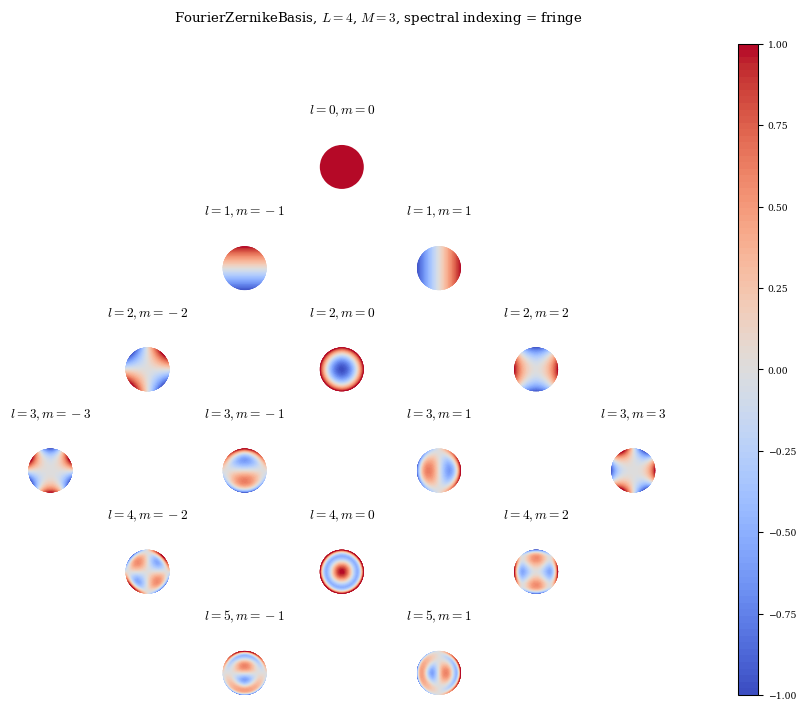
\includegraphics[width=\textwidth,height=8cm,keepaspectratio]{figures/fringeL4M3.png}
        \end{figure}
    \end{minipage}
    \begin{minipage}[t][6cm][t]{0.5\textwidth}
        \begin{figure}[H]
            \centering
            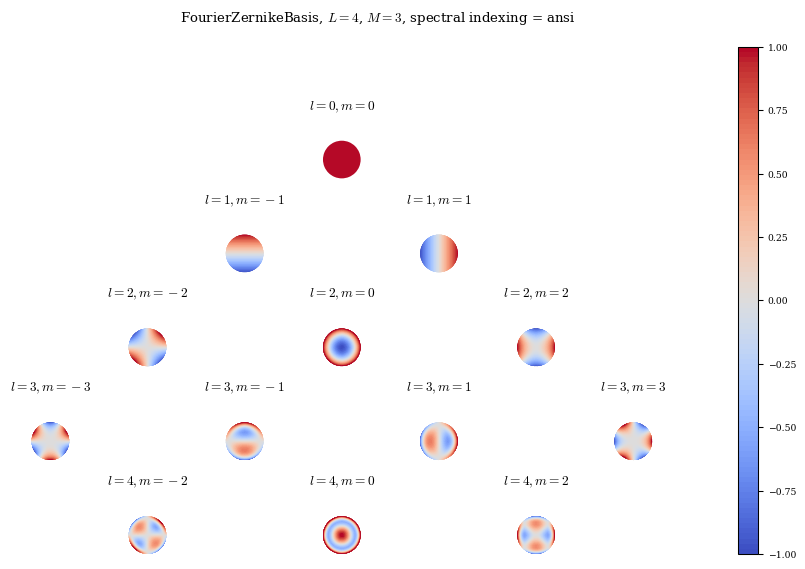
\includegraphics[width=\textwidth,height=8cm,keepaspectratio]{figures/ansiL4M3.png}
        \end{figure}
    \end{minipage}
\end{minipage}
\begin{minipage}[c][8cm][c]{\textwidth}
    \begin{minipage}[t][6cm][t]{0.5\textwidth}
        \begin{figure}[H]
            \centering
            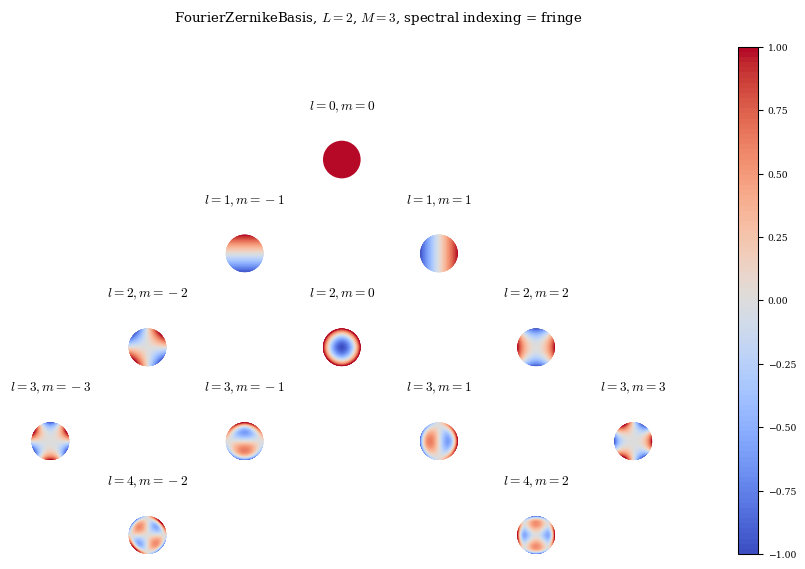
\includegraphics[width=\textwidth,height=8cm,keepaspectratio]{figures/fringeL2M3.png}
        \end{figure}
    \end{minipage}
    \begin{minipage}[t][6cm][t]{0.5\textwidth}
        \begin{figure}[H]
            \centering
            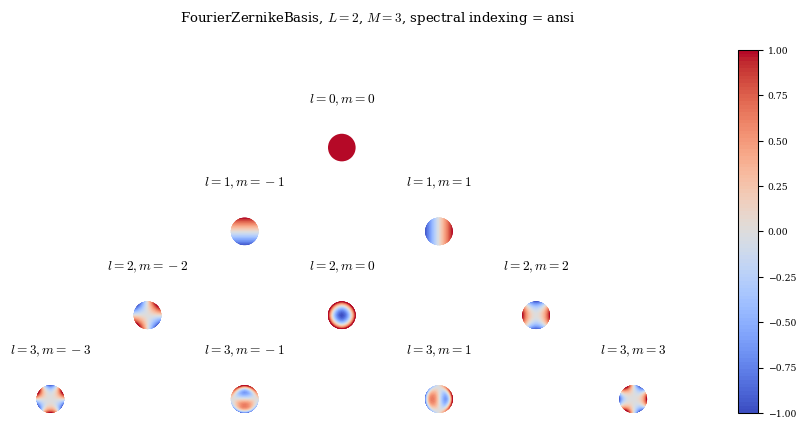
\includegraphics[width=\textwidth,height=8cm,keepaspectratio]{figures/ansiL2M3.png}
        \end{figure}
    \end{minipage}
\end{minipage}
\pagebreak

You can test different cases with the following code block,
\begin{minted}[fontsize=\footnotesize]{python}
    from desc.basis import FourierZernikeBasis
    from desc.plotting import plot_basis
    basis = FourierZernikeBasis(L=4, M=3, N=0, spectral_indexing="ansi")
    plot_basis(basis);
\end{minted}







% ==========================================================================================================================================







\subsubsection{Symmetry Options}
"cos" symmetry doesn't have any sin terms, so only $m>=0$ terms are considered. Similarly, "sin" symmetry doesn't have any cos terms, so only $m<0$ terms are considered.

\begin{minipage}[c][9cm][c]{\textwidth}
    \begin{minipage}[t][9cm][t]{0.45\textwidth}
        \begin{figure}[H]
            \centering
            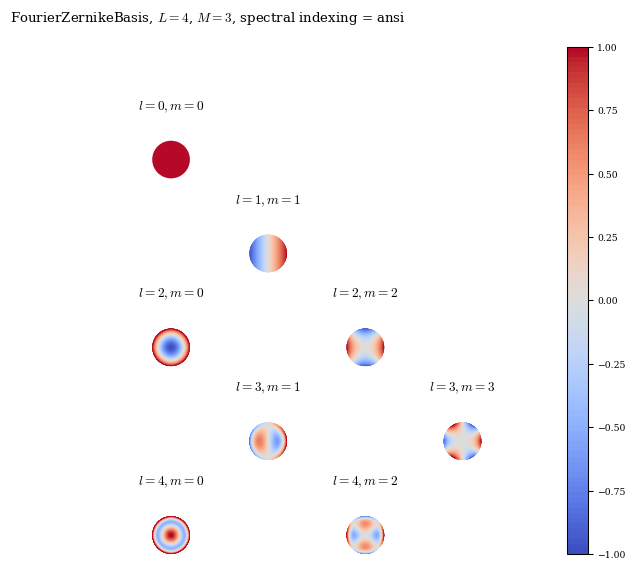
\includegraphics[width=\textwidth,height=8cm,keepaspectratio]{figures/ansiL4M3cos.png}
            \caption{"cos" Symmetry Modes}
        \end{figure}
    \end{minipage}
    \begin{minipage}[t][9cm][t]{0.55\textwidth}
        \begin{figure}[H]
            \centering
            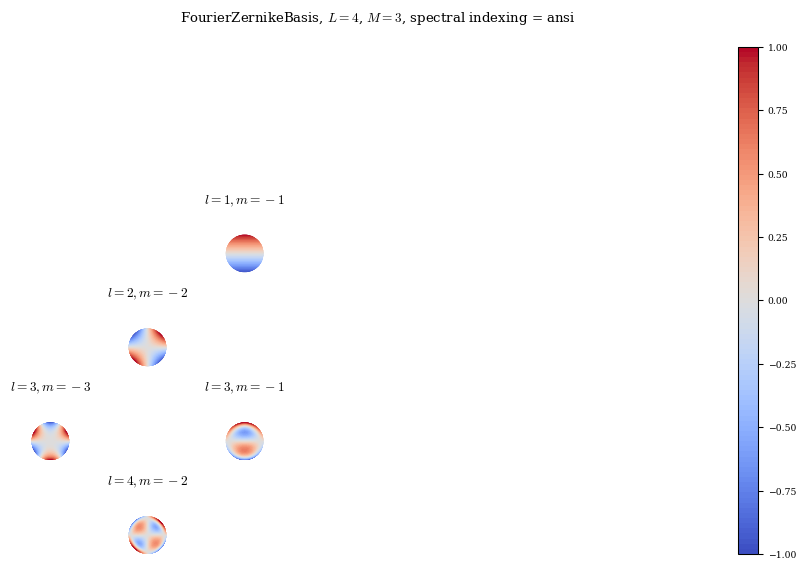
\includegraphics[width=\textwidth,height=8cm,keepaspectratio]{figures/ansiL4M3sin.png}
            \caption{"sin" Symmetry Modes}
        \end{figure}
    \end{minipage}
\end{minipage}

We can find the total number of Zernike modes for \textbf{sym="cos"}, \textbf{spectral\_indexing="ansi"} and $M=L$,
\begin{equation}
    \textit{Total Number of Zernike Modes} \hspace{0.5cm} = \hspace{0.5cm} \mathlarger{\mathlarger{\sum}}_{l=even}^{M} \hspace{0.2cm} \left(\cfrac{l}{2}+1\right) + \mathlarger{\mathlarger{\sum}}_{l=odd}^{M} \hspace{0.2cm} \cfrac{l+1}{2}
\end{equation}
So,
\begin{equation}
    \begin{split}
        \textit{Total Number of Zernike Modes} \hspace{0.5cm} &= \hspace{0.5cm} \begin{cases}
            \hspace{0.2cm}\mathlarger{\mathlarger{\sum}}_{k=0}^{M/2} \hspace{0.2cm} \left(\cfrac{2k}{2}+1\right) + \hspace{0.2cm}\mathlarger{\mathlarger{\sum}}_{k=0}^{M/2-1} \hspace{0.2cm} \cfrac{(2k+1)+1}{2}  &\text{for $M$ even} \\[0.5cm]
            \mathlarger{\mathlarger{\sum}}_{k=0}^{(M-1)/2} \hspace{0.1cm} \left(\cfrac{2k}{2}+1\right) + \mathlarger{\mathlarger{\sum}}_{k=0}^{(M-1)/2} \hspace{0.2cm} \cfrac{(2k+1)+1}{2}  &\text{for $M$ odd} 
        \end{cases}   \\[.5cm]
        &= \hspace{0.5cm} \begin{cases}
            \left(\cfrac{M}{2}+1\right) + \cfrac{(\frac{M}{2}+1)\frac{M}{2}}{2} + \cfrac{M}{2} + \cfrac{(\frac{M}{2}-1)\frac{M}{2}}{2}  &\text{for $M$ even} \\[0.5cm]
            2 \left(\cfrac{M-1}{2}+1 + \cfrac{\frac{M-1}{2}(\frac{M-1}{2}+1)}{2} \right)&\text{for $M$ odd} 
        \end{cases}  
    \end{split}
\end{equation}
\begin{equation}
    \textit{Total Number of Zernike Modes} \hspace{0.5cm} = \hspace{0.5cm} \begin{cases}
        \cfrac{M^2 + 2M + 4}{4}  &\text{for $M$ even} \\[0.2cm]
        \cfrac{M^2 + 4M + 3}{4} &\text{for $M$ odd} 
    \end{cases} 
\end{equation}

Similarly, we can find the total number of Zernike modes for \textbf{sym="sin"}, \textbf{spectral\_indexing="ansi"} and $M=L$,
\begin{equation}
    \textit{Total \# of Zernike Modes} \hspace{0.5cm} = \hspace{0.5cm} \mathlarger{\mathlarger{\sum}}_{l=even}^{M} \hspace{0.2cm} \cfrac{l}{2} \hspace{0.2cm}+ \mathlarger{\mathlarger{\sum}}_{l=odd}^{M} \hspace{0.2cm} \left(\cfrac{l+1}{2} - 1\right)
\end{equation}
\begin{equation}
    \textit{Total \# of Zernike Modes} \hspace{0.5cm} = \hspace{0.5cm} \begin{cases}
        \cfrac{M^2 + 3}{4}  &\text{for $M$ even} \\[0.2cm]
        \cfrac{M^2 + 2M}{4} &\text{for $M$ odd} 
    \end{cases}  
\end{equation}

If we add the number of modes for sin and cos, we can get the total number of modes for \textbf{spectral\_indexing="ansi"} and $M=L$,

\begin{equation}
    \textit{Total \# of Zernike Modes}  =  \begin{cases}
        \cfrac{2M^2 + 2M + 7}{4}  &\text{for $M$ even} \\[0.2cm]
        \cfrac{2M^2 + 6M + 3}{4} &\text{for $M$ odd} 
    \end{cases}  
\end{equation}